%% LaTeX Beamer presentation template (requires beamer package)
%% see http://latex-beamer.sourceforge.net/
%% idea contributed by H. Turgut Uyar
%% template based on a template by Till Tantau
%% this template is still evolving - it might differ in future releases!

\documentclass{beamer}

\mode<presentation>
{
\usetheme{Warsaw}

\setbeamercovered{transparent}
}
\usepackage[english]{babel}
\usepackage[latin1]{inputenc}

% font definitions, try \usepackage{ae} instead of the following
% three lines if you don't like this look
\usepackage{mathptmx}
\usepackage[scaled=.90]{helvet}
\usepackage{courier} 

\usepackage{graphicx}

\usepackage[T1]{fontenc}

 
\title{Scenario Variability Management}
\subtitle{A Controlled Experiment}

\subtitle{A Controlled Experiment}

% - Use the \inst{?} command only if the authors have different
%   affiliation.
%\author{F.~Author\inst{1} \and S.~Another\inst{2}}
\author{Rodrigo Bonif\'{a}cio\inst{1} \and Paulo Borba\inst{1} \and Cristiano
Ferraz\inst{2}}

% - Use the \inst command only if there are several affiliations.
% - Keep it simple, no one is interested in your street address.
\institute[Federal University of Pernambuco]
{
\inst{1}%
Informatics Center
\and
\inst{2}%
Department of Statistics}

\date{Date / Occasion}


% This is only inserted into the PDF information catalog. Can be left
% out.
%\subject{Talks}



% If you have a file called "university-logo-filename.xxx", where xxx
% is a graphic format that can be processed by latex or pdflatex,
% resp., then you can add a logo as follows:

% \pgfdeclareimage[height=0.5cm]{university-logo}{university-logo-filename}
% \logo{\pgfuseimage{university-logo}}

\begin{document}

\begin{frame}
\titlepage
\end{frame}

\begin{frame}
\frametitle{General Objective of the Experiment}
Measure different responses of PLUSS and
mSVCM according to the extractive and reactive
approaches for SPL development
\end{frame}

\begin{frame}
\frametitle{Hypothesis}
\begin{itemize}
\item h1. MSVCM reduces scattering and tangling
\item h2. MSVCM requires less time to evolve
\item h3. MSVCM adheres to the open-close principle
\item h4. MSVCM requires more time to specify a SPL
\end{itemize}
\end{frame}

\begin{frame}
\frametitle{Design of the experiment}
\begin{block}{Two Phases}
 \begin{itemize}
  	\item extract a PL from existing products
	\item evolve an existing PL based on CRs (h1, h2, h3)
 \end{itemize}
\end{block}  	
\begin{block}{Input data for the design activiy}
 \begin{itemize}
  	\item number of students (~18)
	\item number of experimental unities (2)
	\item number of treatments (2)
 \end{itemize}
\end{block}  	

\end{frame}

\begin{frame}
\frametitle{Design of the experiment}
\begin{itemize}
 \item (treatments) == (experimental unities) $\Rightarrow$ Latin
 Square Design
 \item Requires subjects randomly organized in groups
 of two students
 \item If all students were present, 9 replications. As
 greater the number of replication is, the greater
 is the confidence interval
\end{itemize}
\end{frame}

\begin{frame}
\frametitle{Design of the experiment}
Latin Squares for the first experiment
 \begin{center}
 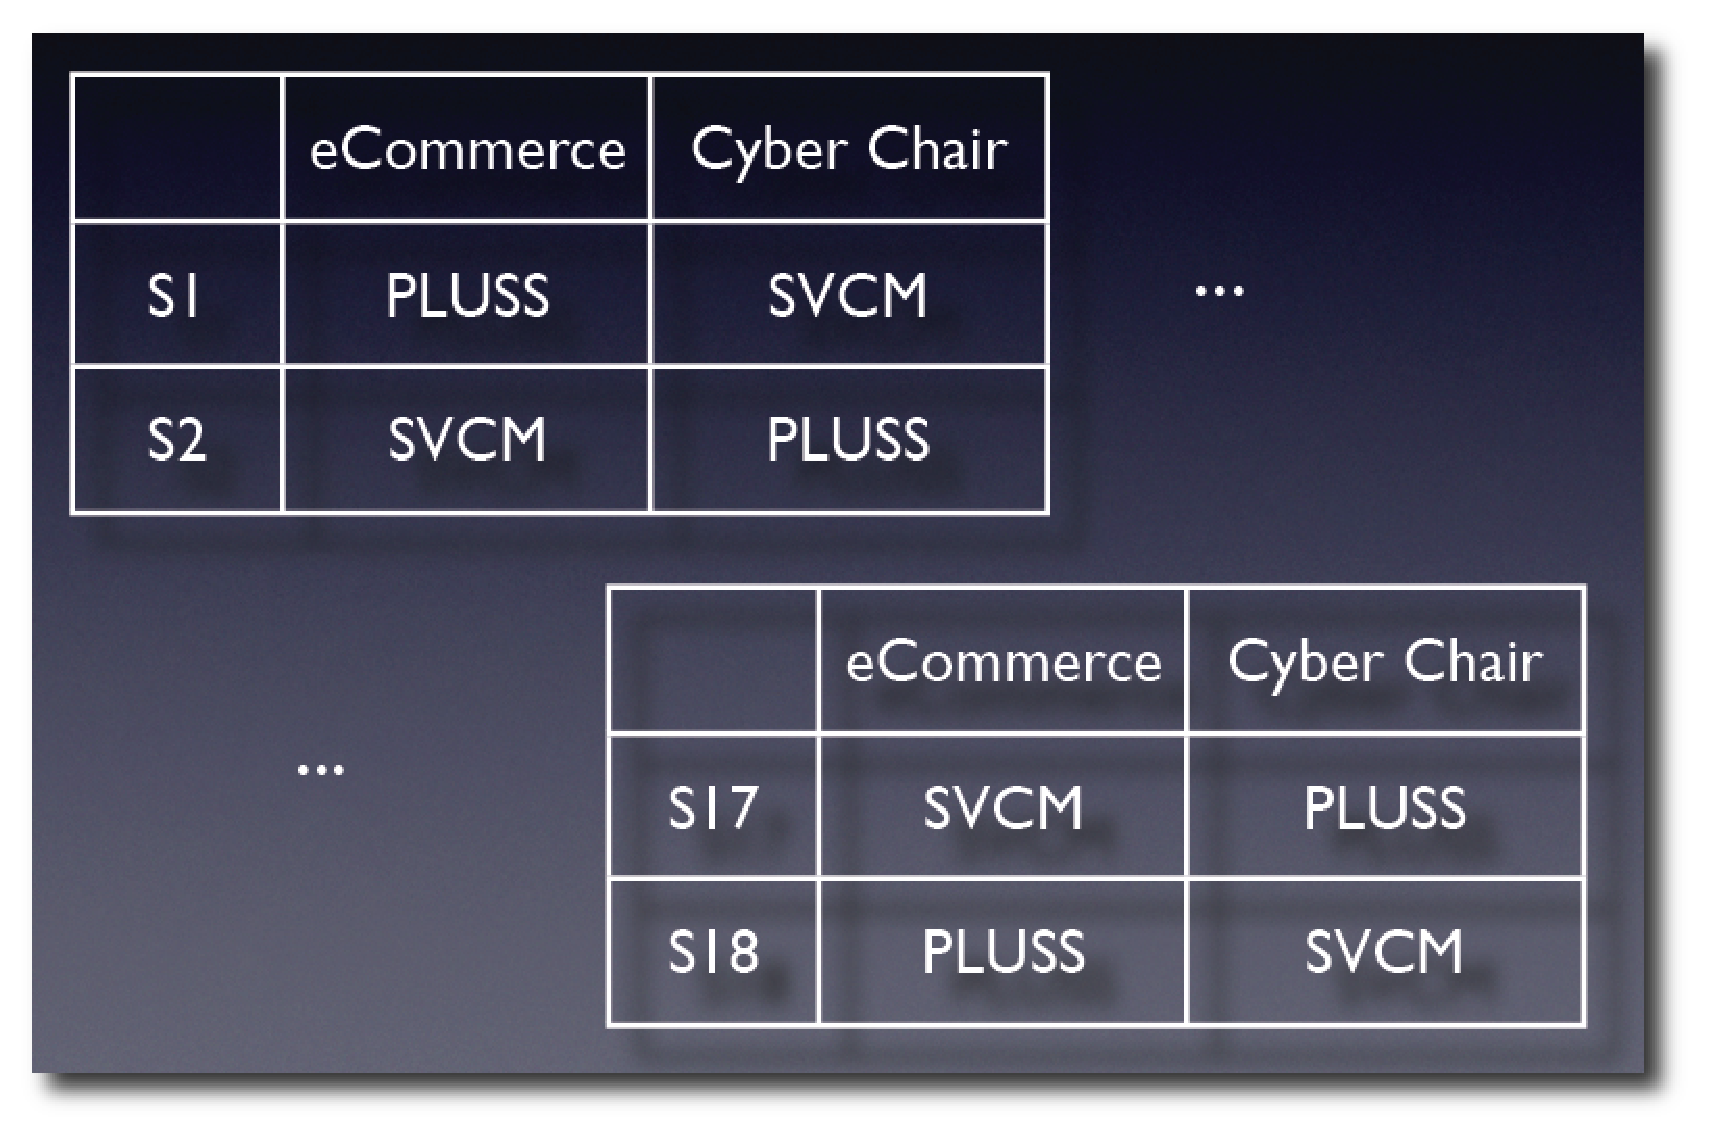
\includegraphics[scale=0.25]{images/lsquare01.eps}
 \end{center}
\end{frame}

\begin{frame}
\frametitle{Design of the experiment}
Latin Squares for the second experiment
\begin{center}
 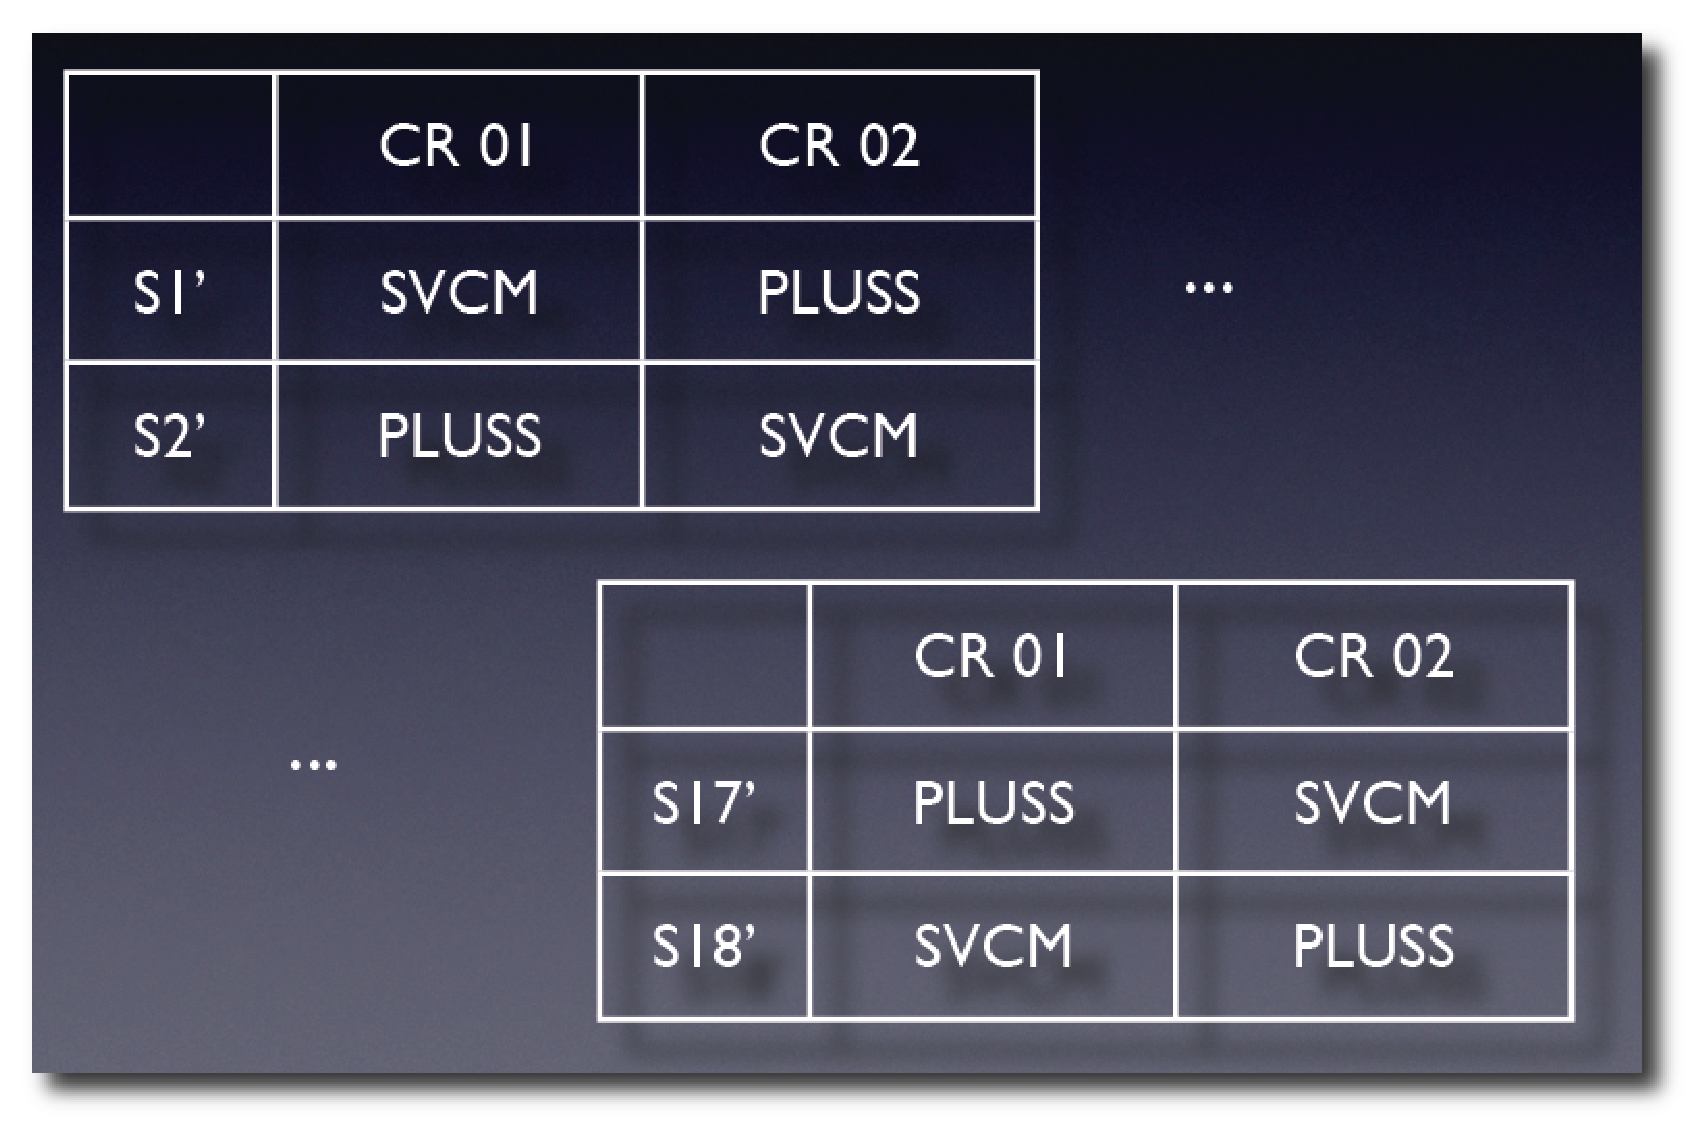
\includegraphics[scale=0.25]{images/lsquare02.eps}
\end{center}
\end{frame}

\begin{frame}
\frametitle{Design of the experiment}
\begin{block}{Additive model}
\center{$Y_{ijt} = \eta + \beta_i + \gamma_j + \tau_t + \epsilon_{ijt} $} 
\begin{scriptsize}
\begin{itemize}
  \item $\eta$ is the mean
  \item $\beta_i$ are the $i = 1 .. k$ row effects
  \item $\gamma_j$ are the $j = 1 .. k$ column effects
  \item $\tau_t$ are the $t = 1 .. k$ treatment effects
\end{itemize}
\end{scriptsize}
\end{block}

\begin{block}{Assumptions}
\begin{itemize}
  \item the errors $\epsilon_{ijt}$ are $IIDN(0,\sigma^2)$
  \item The model must be additive
\end{itemize}
\end{block}

\end{frame}

\begin{frame}
\frametitle{Analysis Procedure}
\begin{enumerate}
  \item Check if the results comply to the model assumptions
  \item Check if the treatments are relevant to the response variable
  \item Identify the best option among the treatments 
  \begin{itemize}
    \item Two treatments: compare the mean values
    \item Otherwise: perform multiple comparsions among the treatments
    (different techniques, such as Fisher and Tukey)
  \end{itemize}
\end{enumerate}
\end{frame}
\end{document}

\begin{frame}
\frametitle{Analysis Procedure}
\begin{block}{Check the model assumptions}

\end{block}
\end{frame}
\end{document}